\section{Network Characteristics of Notification Services}
\label{sec:characterize-os}

Mobile operating systems provide OS level notification services to optimize network usage.
The Apple Push Notification service (APNs)~\cite{apns} and Google Cloud Messaging (GCM)~\cite{gcm} are used by iOS and Android applications respectively to receive notifications from the Internet.
In this section we show how \platname was used to compare the notification services of iOS and Android, and detailing it behavior in the wild. 

\begin{figure}
\centering
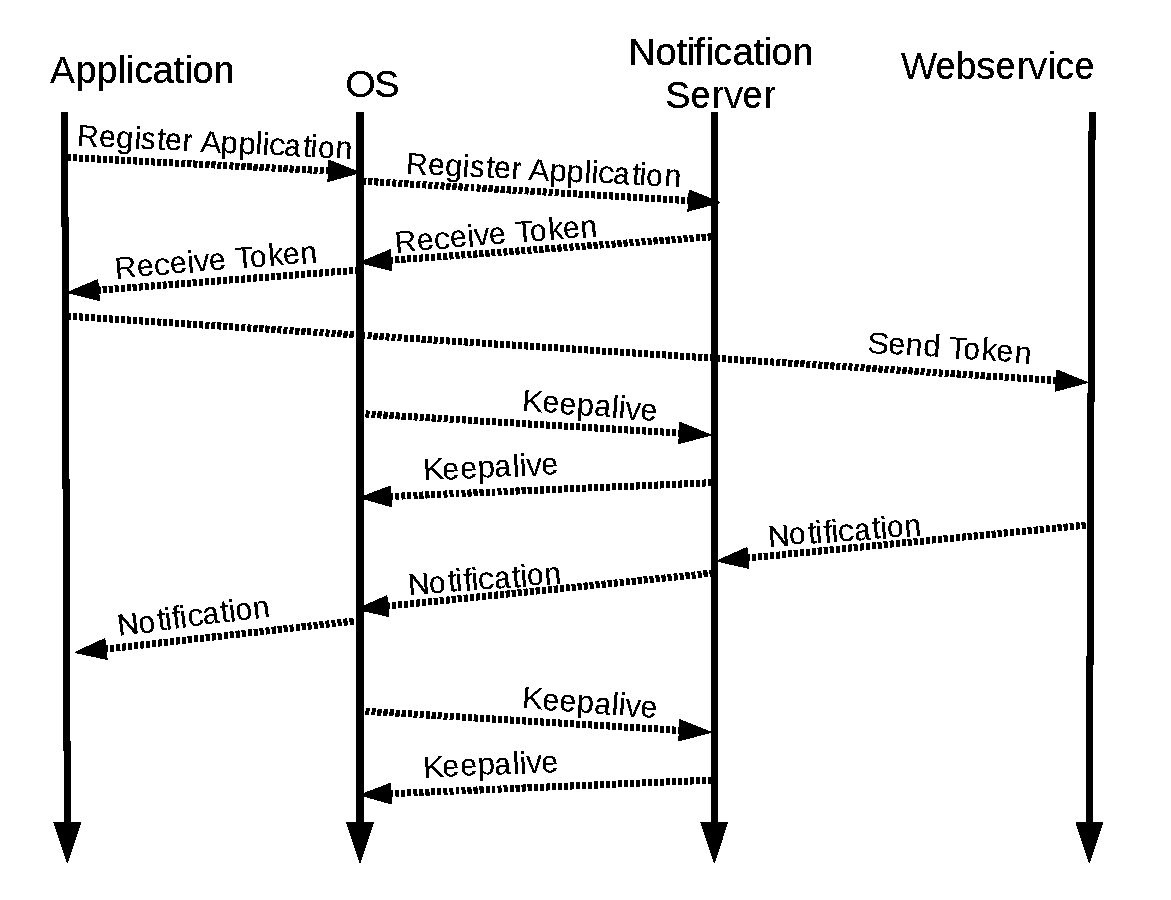
\includegraphics[width=0.8\columnwidth]{figures/Notification.pdf}
\caption{Notifications on mobile OSes. \emph{Periodic keepalive messages ensure that TCP connections do not time out.}}
\label{fig:push-expt-interarrival}
\end{figure}

In \fref{fig:push-expt-interarrival}, we show how the iOS and Android devices use TCP to receive notifications from their respective notification servers. 
These notification servers aggregate notification messages from various web-services that want to push messages to the devices.
As shown in \fref{fig:push-expt-interarrival}, the application that is allowed to receive notifications first registers itself and obtains a token from the notification server.
This token is then shared with the Web-service from which the application desires to receive notifications. 
The Web-service uses this token to specify the device and the application to which notification messages are to be sent. 
On receiving a notification message, the notification server forwards the notifications based on its forwarding policies~\cite{apns, gcm}. 
A dedicated OS service is responsible for receiving the notifications on the mobile device and sending them to the application.
This service periodically sends keepalive messages to ensure that the TCP connection does not time out.
The notification services for iOS use port 5223 and port 5228 on Android~\cite{apns, gcm}.
The notification messages do not depend on user activity, therefore, they represent the minimum data traffic that any device can generate.

\subsection{Controlled Experiment on Factory Reset Devices}

To shed light on the network characteristics of notification services we perform a controlled experiment on \emph{factory-reset} devices. 
Our goal was to analyze notification services on devices used \emph{out of the box}, and detail the impact of device manufacturer, access technology, and pre-installed applications. 

We began our experiment by first performing a \emph{factory reset} on a fully charged iPod Touch, iPad, iPhone, a Samsung Galaxy SIII, and a Google Nexus S Phone.
We then initialized the devices with a dummy email account and observed its \wifi traffic for 24 hours using \platname.
We then let the iPhone, Google Nexus~S, and Samsung Galaxy SIII connect to the Internet using their cellular interface for 24 hours to detail the impact of access technology.

The factory reset ensured that these devices generated very little traffic, from 19~KB to 97~KB depending on the device. 
We filter out the notification messages in our traces using the TCP port numbers and AS mentioned in their respective specifications~\cite{gcm, apns}.
Indeed, notification messages were responsible for largest fraction of the traffic volume; the share was 35\% for Nexus S, 88\% for the Samsung SIII and around 50\% for each of the iOS devices. 
The rest of the traffic was primarily due to DNS requests made by the device. 
%The share of DNS traffic varied from 10\% to 40\% for each of the devices while the other services contributed to less than 10\% of the traffic volume.
%The only exception was the Samsumg Galaxy SIII which used location services that contributed to 26\% of 47~KB traffic volume generated by the device.

\begin{figure}
\centering
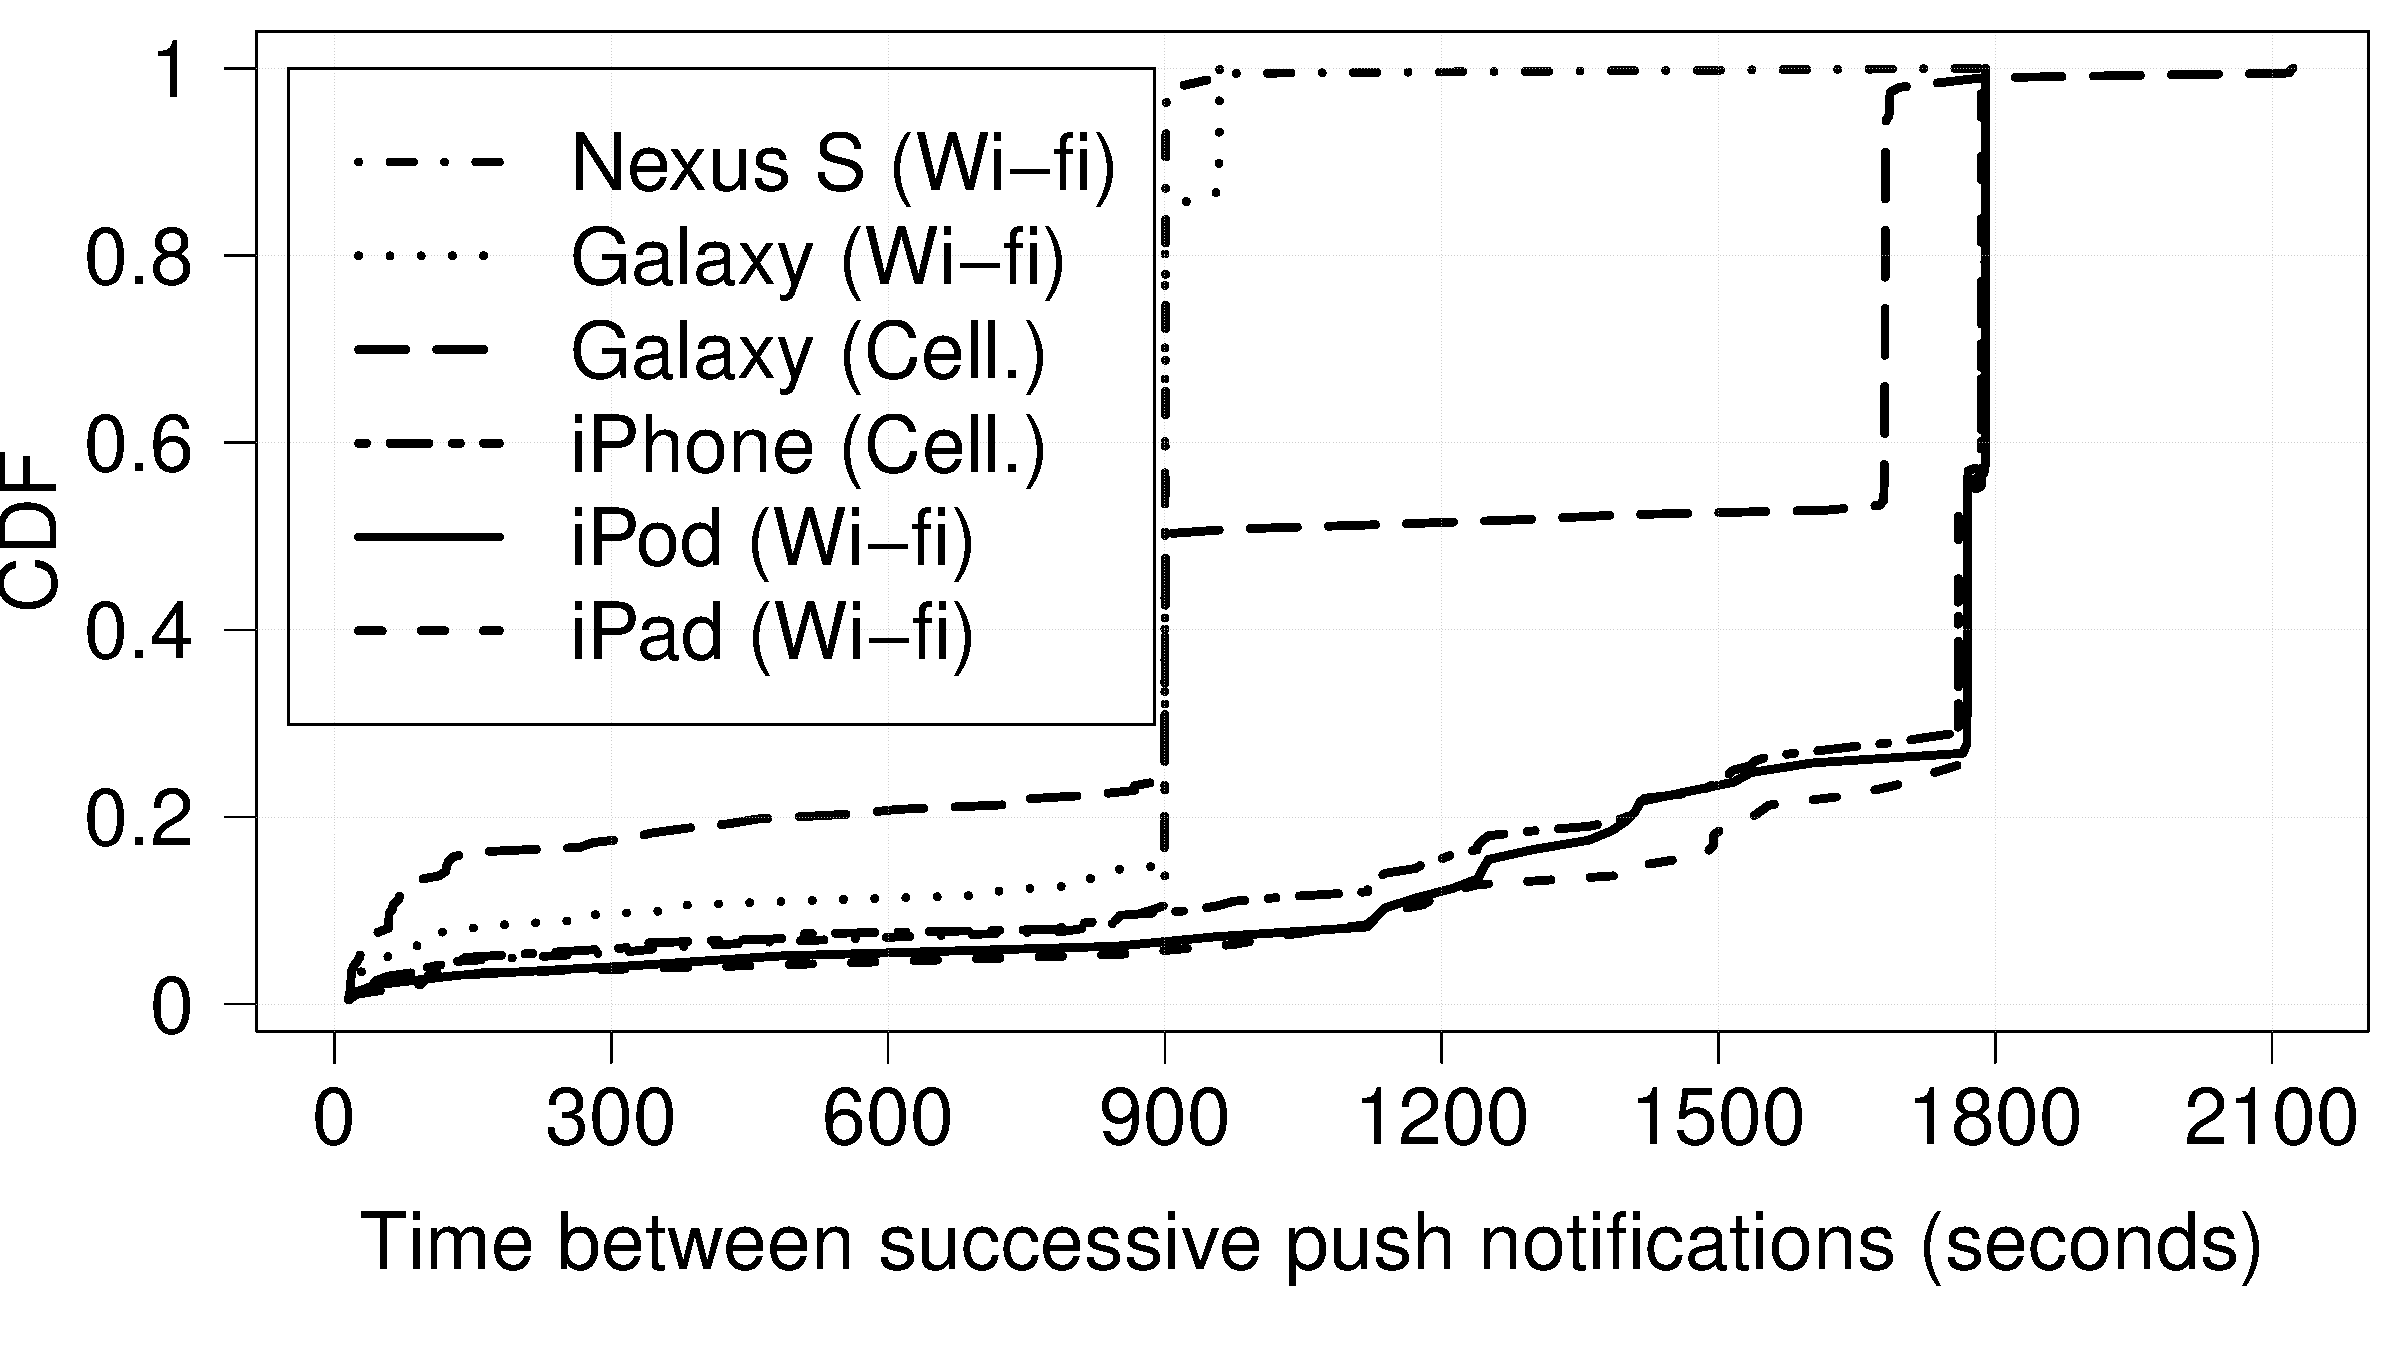
\includegraphics[width=\columnwidth]{plots/push_factoryreset_interarrival_distrib.pdf}
\caption{Inter-arrival time between notification messages after factory reset. \emph{The Android and iOS devices communicate with the notification server approximately once every 900~seconds and 1800 seconds respectively. The behavior of Android devices depends on the device, the pre-installed applications, and the access technology.}}
\label{fig:push-expt-interarrival}
\end{figure}

To detail the behavior of keepalive, we plot the time between successive messages in \fref{fig:push-expt-interarrival}.
We observe that more than 75\% of the messages are sent after an idle period of 1700~seconds on iOS devices and 900~seconds for Android devices. 
Furthermore, we observe that behavior for the Samsung Galaxy SIII depends on the access technology.
Due to lack of space we do not present the results for Nexus-S and iPhone for which we did not observe any impact of access technology.

On inspecting the packets exchanges, we observe that iOS messages with an inter-arrival time larger than 1500 seconds began with an TCP packet with a payload of 85 bytes sent by the device followed by the server responding with of a TCP packet of 37 byte payload.
Similarly, Android flows with an inter-arrival time larger than 800 seconds consisted of an empty TCP packet sent by the device followed by a 25 byte payload sent by the server.
We speculate these messages to be keepalive messages.

In summary, we observe notifications consume very little data, less than 50~KB in 24 hours, on Android and iOS devices in their default state.
The large time between successive notifications and the small amount of data exchanged implies they consume very little power.
We also observe that iOS devices have a larger time between successive notifications compared to Android devices in the default state. 
Furthermore, the inter-arrival time between notifications for Android devices differs based on the device manufacturer and the access technology. 

\subsection{Notifications In The Wild} 

We now detail the frequency, traffic volume, and source of the notification services we observed in the \mobWild dataset. 

\begin{figure}
\centering
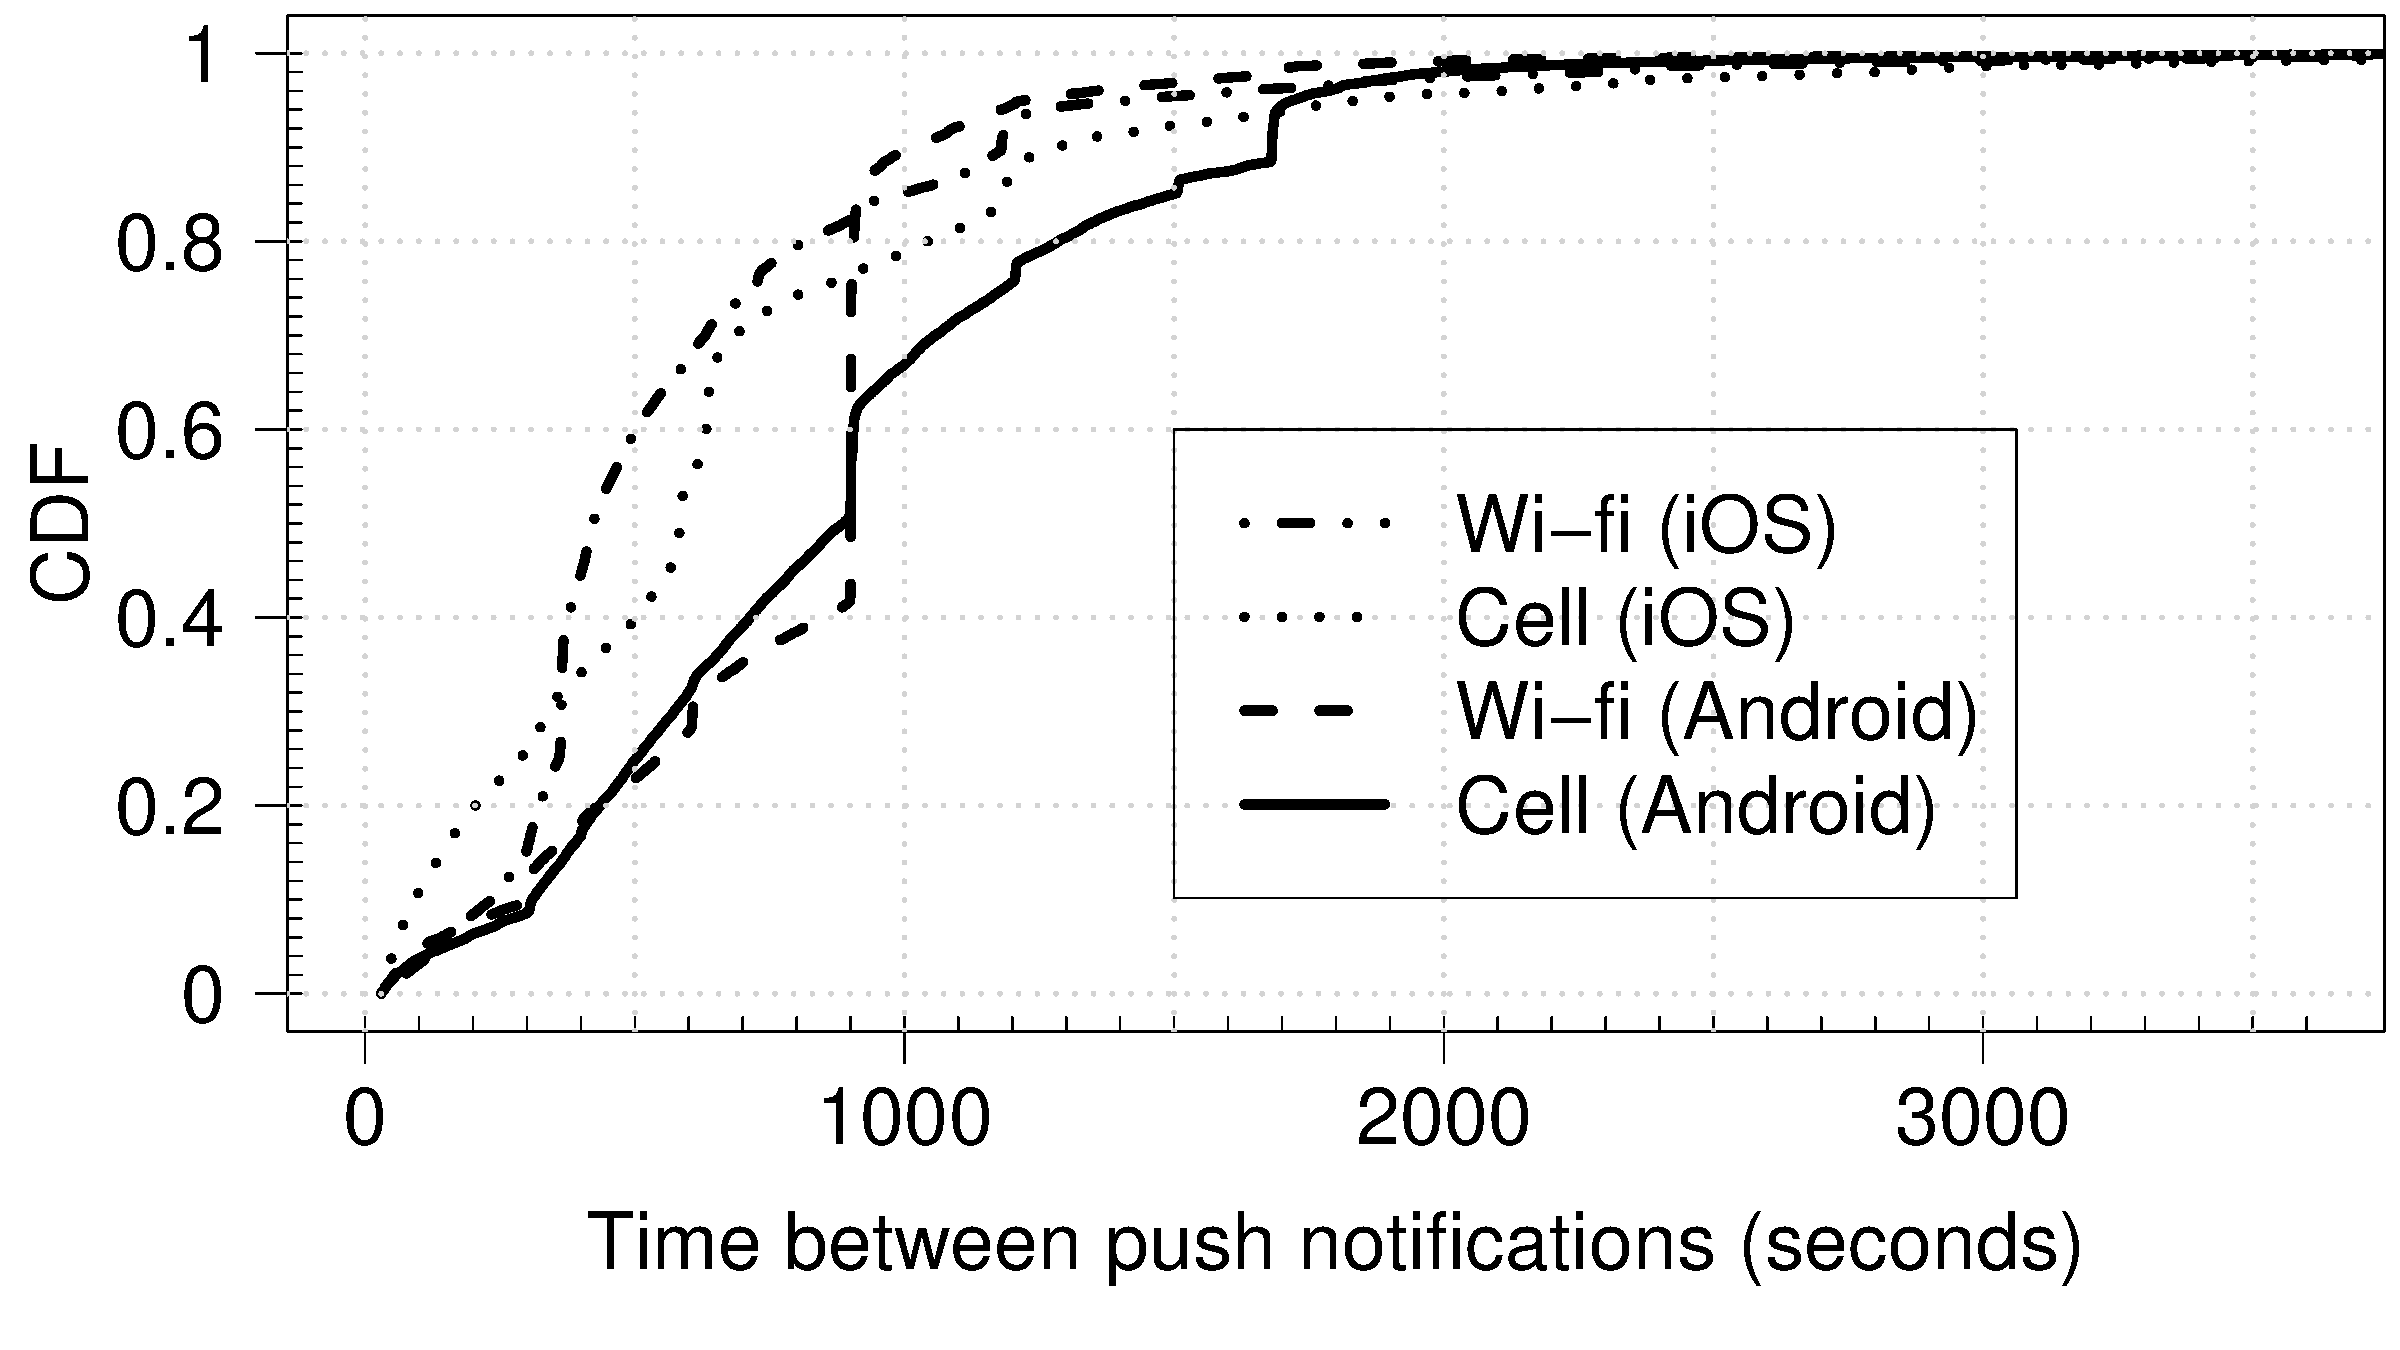
\includegraphics[width=\columnwidth]{plots/push_compare_os_tech_wild_distrib.pdf}
\caption{Distribution of the time between push notification messages in the wild. \emph{The frequency of push notification messages is higher for the iOS devices in our dataset compared to the Android devices. Notification messages are less frequent over cellular networks compared to Wi-Fi networks.}}
\label{fig:push-wild-compare-ostech}
\end{figure}

To analyze the frequency of notification messages, we plot the distribution of the time between successive push notification messages for iOS and Android devices over cellular and \wifi networks in \fref{fig:push-wild-compare-ostech}.
In \fref{fig:push-wild-compare-ostech} we observe that a higher time between push notifications over cellular networks in comparison to \wifi networks for iOS and Android devices.  
We also observe the Android devices in our dataset receive notifications less frequently compared to the iOS devices in our dataset. 
We also observe a heavy tail for the time between notification messages which implies potentially long idle intervals.


\begin{figure}
\centering
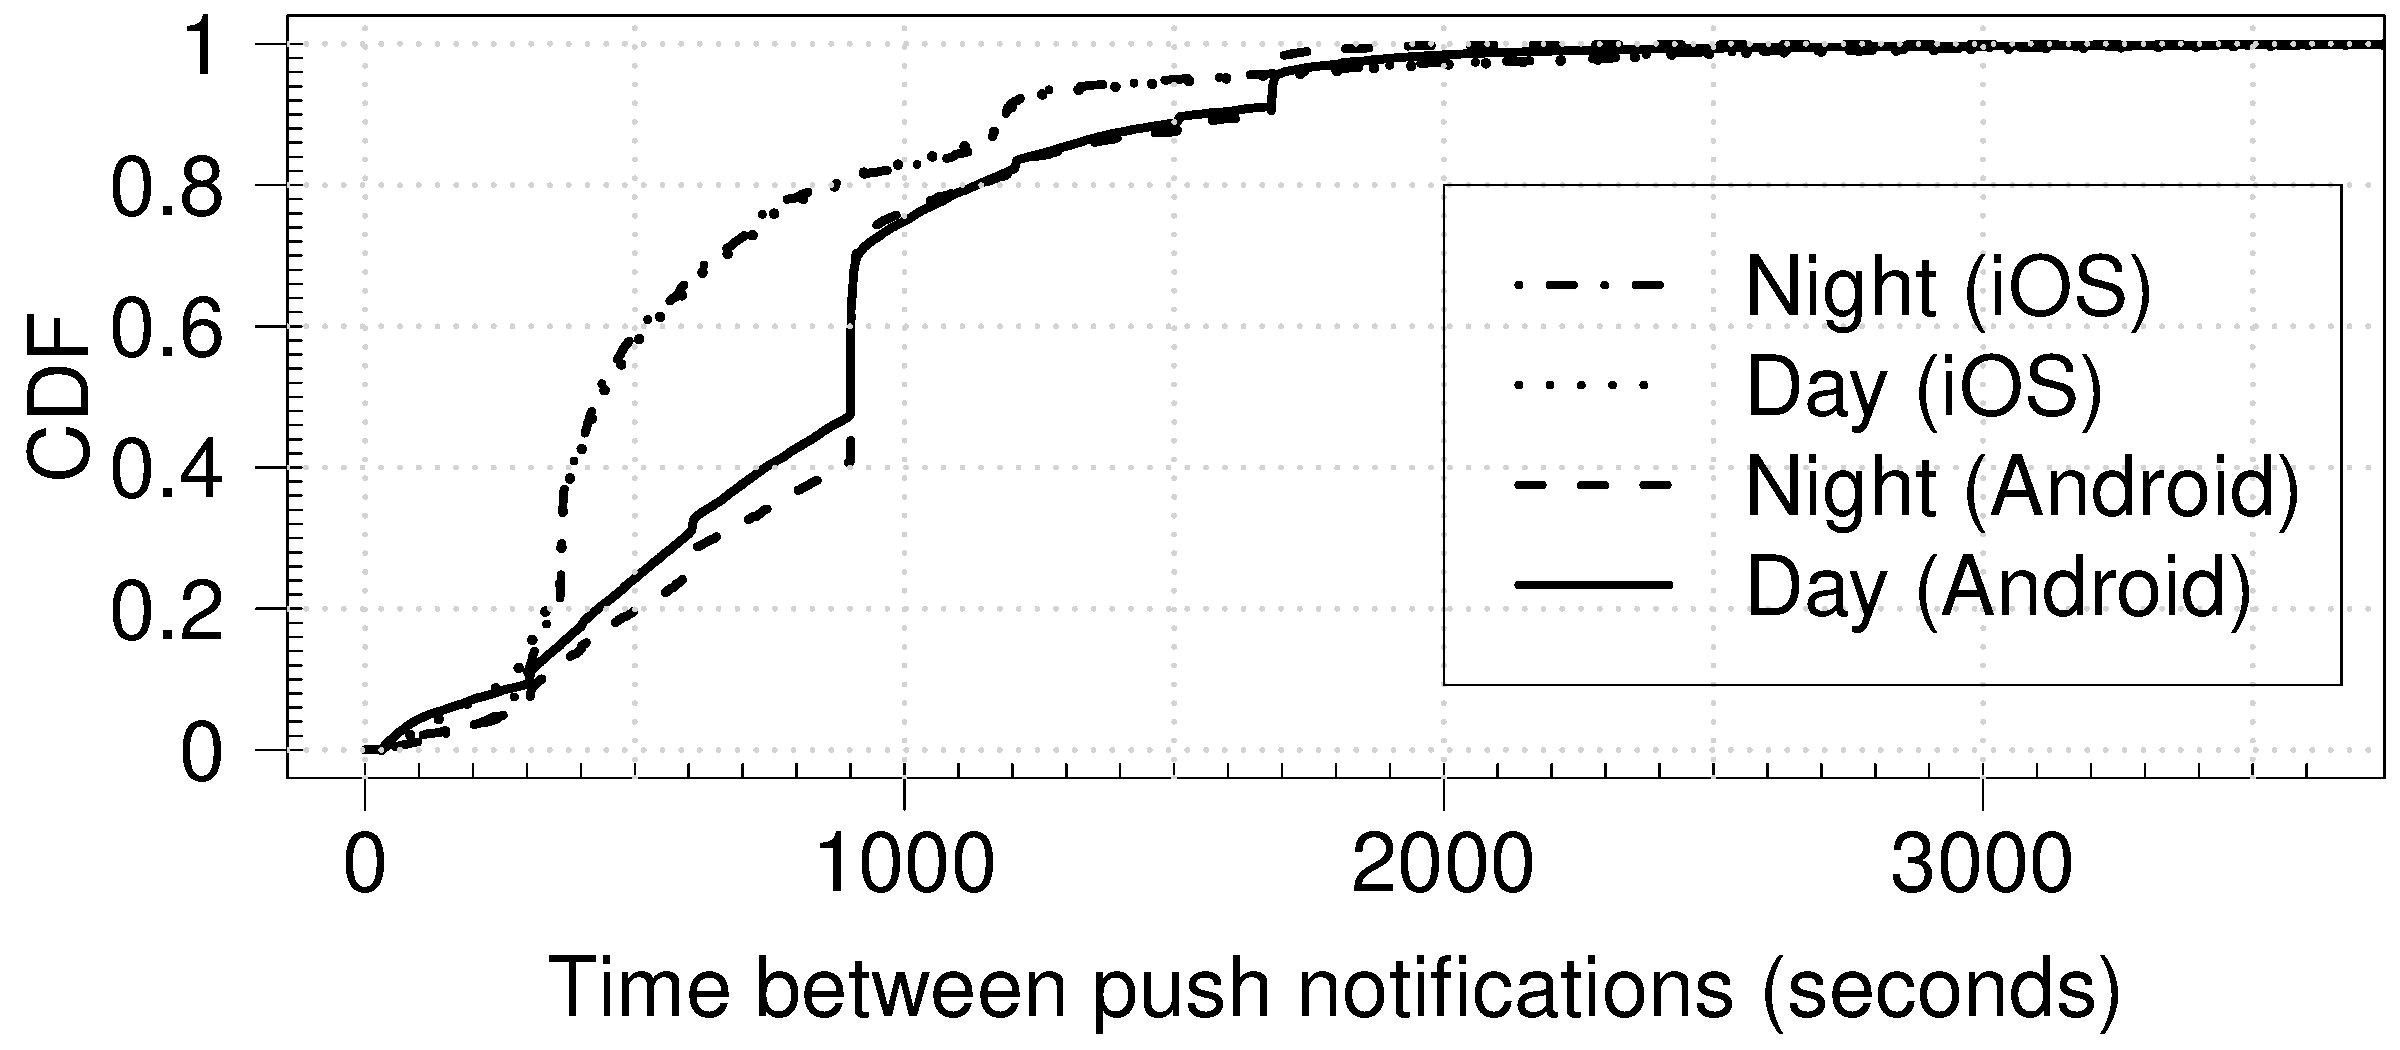
\includegraphics[width=\columnwidth]{plots/push_compare_diurnal_wild_distrib.pdf}
\caption{Impact of time-of-day on the push notifications. \emph{The rate of notifications is agnostic of the time of the day for iOS and Android devices.}}
\label{fig:push-wild-diurnal}
\end{figure}

The notification messages could be in response to user actions, for example, a mail server might receive a notification of a new message.
To analyze this impact, we notification messages received during two time intervals: from midnight to 6 am (night), and from 6 am to midnight (day). 
In \fref{fig:push-wild-diurnal}, we plot the distribution between successive notification messages for these two intervals. 
We observe that the Android and iOS devices appear to be agnostic of the time of the day. 
The iOS devices (from verion 6.0) come with a feature called \emph{Do Not Disturb (DND)} that does raise notification alarms on receiving notifications during specific time periods. 
We observe notification messages were received by the device that had enabled this feature during the intervals their users had configured as \emph{Do Not Disturb}.

Despite the periodic nature of notification messages, in \fref{tab:classify-ssl-port} we observe that notification messages are responsible for less than 2\% of the SSL traffic from iOS and Android devices\footnote{We observe similar fraction for notification messages from each device and also for each access technologies used by the device, we do not present these results due to lack of space}.
We then used the DNS requests to identify the servers that pushed notifications.
We observe that these request match the pattern \emph{*courier.push.apple.com} and \emph{*courier-push-apple.com.akadns.net} for the iOS devices and \emph{*talk.google.com} for Android devices. 

In summary, we detail the behavior of the notification services using controlled experiments and the \mobWild dataset.  
We observe that push notifications consume a small fraction of the data and exhibit a heavy tail for the time between successive messages. 
We also observe that the frequency of notification messages was agnostic of the time of the day. 
Furthermore, notification messages were received by iOS devices even during the time interval the users had configured \emph{Do Not Disturb.}


%%% Local Variables: 
%%% mode: latex
%%% TeX-master: "main.tex"
%%% End: 

% \begin{packedenumerate}
% \item How frequently do Push notifications take place in the wild?
% \item What is the impact of access technology on push notifications?
% \item What is the impact of the time of the day?
% \item What is the volume of push notification traffic?
% \item From which hosts are these notifications received?
% \end{packedenumerate}

%\subsection{Discussion}




% OLD TABLE WITHOUT IPHONE
% \begin{table}
% \begin{small}
% \begin{tabular}{|c|c|c|c|c|}
% \hline
% \multirow{2}{*}{\bf Application} & \multicolumn{4}{c|}{\bf Traffic Share in the first 24 hours}\tabularnewline
% \cline{2-5}
%      & iPad & iPod & Galaxy SIII & Nexus \tabularnewline
%      & (19 KB) & (21 KB) & (47 KB)& (97 KB)  \tabularnewline
% \hline
% Notifications & 0.54 & 0.53 & 0.35 & 0.88 \tabularnewline
% \hline
% Location & 0 & 0 & 0.26 & 0 \tabularnewline
% \hline
% SSL & 0 & 0 & 0.30 & 0.11 \tabularnewline
% \hline
% Mail & 0.05 & 0.07 & 0 & 0 \tabularnewline
% \hline
% HTTP & 0.13 & 0 & 0.09  & 0 \tabularnewline
% \hline
% UDP & 0.28 & 0.40 & 0.01 & 0.01 \tabularnewline
% \hline
% {\em total}& {\em 1.0} & {\em 1.0} & {\em 1.0} & {\em 1.0}\tabularnewline
% \hline
% \end{tabular}
% \end{small}
% \caption{Network usage in the first 24 hours after factory reset. \emph{Notifications contribute to the largest fraction of traffic volume across all devices.}}
% \label{tab:traffic-share-factory-reset}
% \end{table}

%While computing this distribution, we account the diversity in device usage in the following manner.
%For each device and each access technology we compute the 100 quantiles from 0.01 to 1.0 in steps of 0.01 of the time between successive push notifications. 
%We then use the median value of each quantile (from 0.01 to 1.0 in steps of 0.01) for a given access technology and operating system of the device.

% In \fref{fig:wild-inter-arrival-push} we present the time between successive push notifications for the 25 devices in our dataset. 
% As observed in \fref{fig:wild-cdf-push} we observe that the iOS devices receive push messages more frequently that the Android devices. 
% We also observe that the time between push notifications is higher for Android devices.
% The iOS devices prefer a cellular data connection for Push notification over \wifi \tbd{http://support.apple.com/kb/TS4264}. 
% However, in \fref{fig:wild-cdf-push} and \fref{fig:wild-cdf-push} despite this preference, we observe that the time between successive push notifications for iOS devices is higher over cellular networks in comparison to \wifi networks.  
% We observe that \tbd{SSL traffic} to mail servers was followed \tbd{x\%} after push notifications.
% This implies that higher usage of the device over \wifi may result in a higher number of notificatons received. 
% In \fref{fig:wild-inter-arrival-push}, device ID 
%Only if the cellular connection is not available or viable will the device switch to Wi-Fi for APNs connections.

%Furthermore, In \fref{fig:push-traffic-share}, we also plot the share of notification messages when the device exchanged data over cellular networks. 
%We observe that there is no significant difference in the traffic share of notification messages when the device used cellular traffic. 
%\tbd{Why do we care?}

% \begin{figure}
% \centering
% 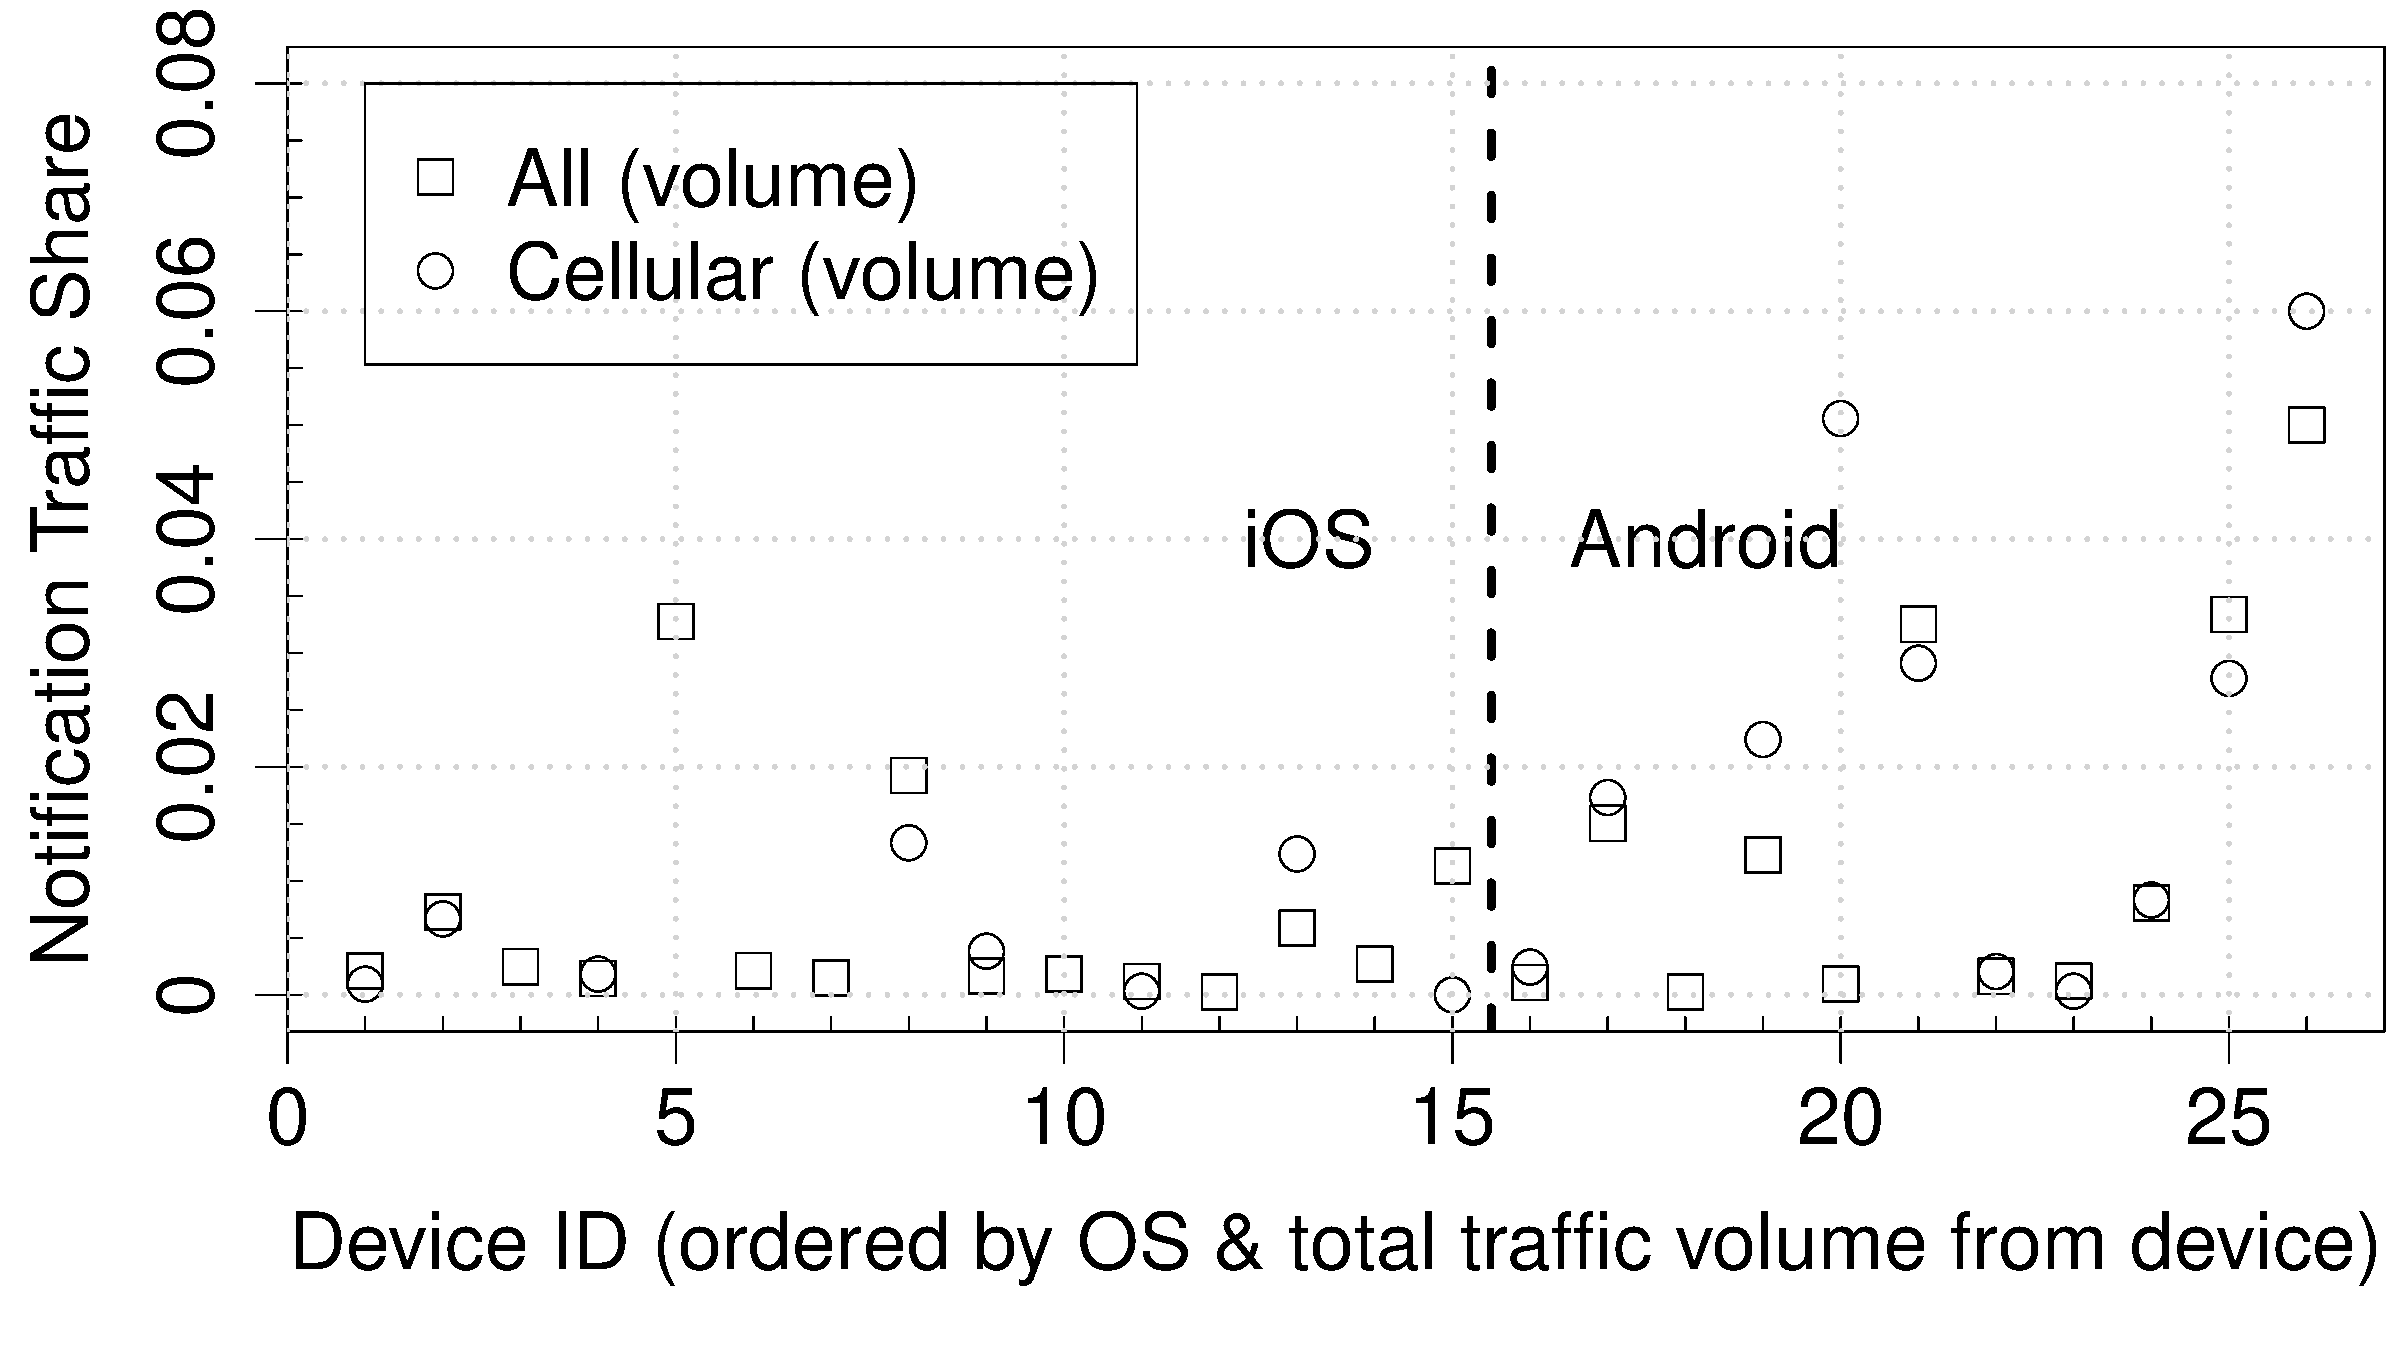
\includegraphics[width=\columnwidth]{plots/push_compare_trafficshare.pdf}
% \caption{Traffic share of push notifications. \emph{Push notifications are responsible for less than 5\% of the traffic volume on most devices.}}
% \label{fig:push-traffic-share}
% \end{figure}
